\documentclass[12pt]{article}
    \usepackage[margin=1in]{geometry}
    \usepackage{mdframed}
    \usepackage{subcaption}
    \usepackage{amssymb}
    \usepackage{amsmath}
    \usepackage{mathtools}

    % Custom colors
    \usepackage{color}
    \definecolor{deepblue}{rgb}{0,0,0.5}
    \definecolor{deepred}{rgb}{0.6,0,0}
    \definecolor{deepgreen}{rgb}{0,0.5,0}
    % Default fixed font does not support bold face
    \DeclareFixedFont{\ttb}{T1}{txtt}{bx}{n}{12} % for bold
    \DeclareFixedFont{\ttm}{T1}{txtt}{m}{n}{12}  % for normal
    \usepackage{listings}
    \usepackage{url}

    \usepackage{hyperref}

    \usepackage{booktabs}
    
    \usepackage{tikz}
    \usetikzlibrary{shapes,arrows,automata,positioning,cd}
    \tikzset{
      cfgedge/.style   = {black, ->, >=stealth},
      forward/.style = { blue, ->, >=angle 45},
      backward/.style = { red, densely dashed, ->, >=latex' },
      backwardleft/.style = { red, densely dashed, <-, >=latex' },
    }
    \usepackage{xcolor}
    
    \newcommand{\cfgarrow}{\mathbin{\tikz[baseline]\draw[cfgedge,yshift=0.6ex] (0,0) -- (.9em,0);}}
    \newcommand{\forwardarrow}{\mathbin{\tikz[baseline]\draw[forward,yshift=0.6ex] (0,0) -- (1em,0);}}
    \newcommand{\backwardarrow}{\mathbin{\tikz[baseline]\draw[backward,yshift=0.6ex] (0,0) -- (.95em,0);}}
  \newcommand{\dom}{\underline{\gg}}
    
    
    \begin{document}
    \lstset{
    language=C,
    basicstyle=\ttfamily\small,
    keywordstyle=\ttb\color{deepblue}\small,
    emph={foo,bar,assert,baz},          % Custom highlighting
    emphstyle=\ttb\color{deepred}\small,    % Custom highlighting style
    stringstyle=\color{deepgreen}\small,
    frame=tb,                         % Any extra options here
    numbers=left,
    stepnumber=1,
    showstringspaces=false            % 
    }
    
    \begin{center}
        \bigskip
        {\LARGE ECS 240 Programming Languages} \medskip
                
        {\Large Homework 3} \bigskip
    
    \end{center}
    
    \section*{About This Assignment}
    

    \begin{itemize}
      \item This assignment tests you on your understanding of dataflow analysis.
      \item To complete the assignment (i)~modify \texttt{hw3.tex}, (ii)~create
      the corresponding PDF document (using pdflatex, for example), and
      (iii)~submit the pdf electronically via Gradescope by the due date; see
      \href{https://www.gradescope.com/get_started#student-submission}{this page}
      and
      \href{http://gradescope-static-assets.s3-us-west-2.amazonaws.com/help/submitting_hw_guide.pdf}{this
      document}. Your assignment will not be graded and you will receive no
      points if you do not follow these instructions. 

      \item \textbf{When submitting the assignment on Gradescope, please mark
      which page corresponds to each question on the assignment.}  Your
      assignment will not be graded and you will receive no points if you do not
      mark the pages.      

      \item The  \LaTeX\ source has \texttt{TODO}~comments to clearly indicate
      where changes need to be made. 
      The \verb=\vspace= commands can be safely commented out.
      \item This assignment can be worked on in a group of at most three. Enter
      the names and email addresses of the team members in the space provided
      below.
      \item You should assume that statements in basic blocks are either
            assignment statements of the form \lstinline$x = y + z$, or function
            calls of the form \lstinline$x = foo(y, z)$ or \lstinline$bar(x,y)$, where \lstinline$x, y, z$ 
            are arbitrary variables. All
            parameters to functions are passed by value.

            More formally, the grammar of the statements can be represented using the following EBNF grammar:
            \begin{align*}
            stmt &::= var\ `=\textrm'\ expr  \mid call \\
            expr &::= var \mid constant \mid var\ op\ var  \\
            op &::= + \mid - \mid *  \\
            call &::= [var\ `=\textrm' ]\ name\ `(\textrm'\ \{var\}\ `)\textrm' 
            \end{align*}
    \end{itemize}

    \begin{mdframed}
      Team members:
      \begin{itemize}
        %TODO
        \item Name, email address % Enter name and email address of first team member.
        \item Name, email address % Comment out this line if working individually.
        \item Name, email address % Comment out this line if working in pairs.
      \end{itemize}
    \end{mdframed}

    \begin{enumerate}


            
        \item (5 points) Given a dataflow analysis framework $(D, V, \wedge, F)$,
        prove that the following two definitions of \emph{monotonicity} are equivalent:
        \begin{itemize}
          \item For all $x$ and $y$ in $V$ and $f \in F$, $x \leq y$ implies $f(x) \leq f(y)$.
          \item For all $x$ and $y$ in $V$ and $f \in F$, $f(x \wedge y) \leq f(x) \wedge f(y)$.
        \end{itemize}

        \begin{mdframed}
          \vspace{2em}
          % TODO
        \end{mdframed}

        \item  (5 point) $G_l$ is a CFG containing 10 basic blocks. \\We know nothing
        about $G_l$ \emph{except} that 
        
        \begin{itemize}
          \item the basic block $B_5$ is:
        \renewcommand{\arraystretch}{1}
        \begin{tabular}{|c|}
          \hline
          \lstinline$y = x $\\
          \hline
        \end{tabular}
        \item the basic block $B_9$ is:
        \renewcommand{\arraystretch}{1}
        \begin{tabular}{|c|}
          \hline
          $d_1: $ \lstinline$x = 5$\\
          \hline
        \end{tabular}
        \item $B_9$ dominates $B_5$.
        \item Definition $d_1$ reaches  $IN[B_5]$.
      \end{itemize}
    
            
      State whether \textbf{True} or \textbf{False}: 
    
      \emph{It is always correct to replace the use of \lstinline$x$ in $B_5$ 
      with the constant 5.}
    
      If \textbf{True}, justify your answer.
      If \textbf{False}, provide an example of the CFG $G_l$ where the replacement is incorrect.
      \begin{mdframed}
      \vspace{3em}
      %% TODO Comment out the correct answer.
      %\textbf{True} % Provide justification.
      %\textbf{False} % Provide counter example.
      \end{mdframed}
        
      
      \clearpage
      \item (10 points) A variable $x$ is said to be \emph{Useful} at a program point $p$ 
      if the value of $x$ at $p$ could be used as the argument to a function call or
      in the definition of a Useful variable along some path in the control-flow graph starting
      at $p$.

      Consider the following control-flow graph:

      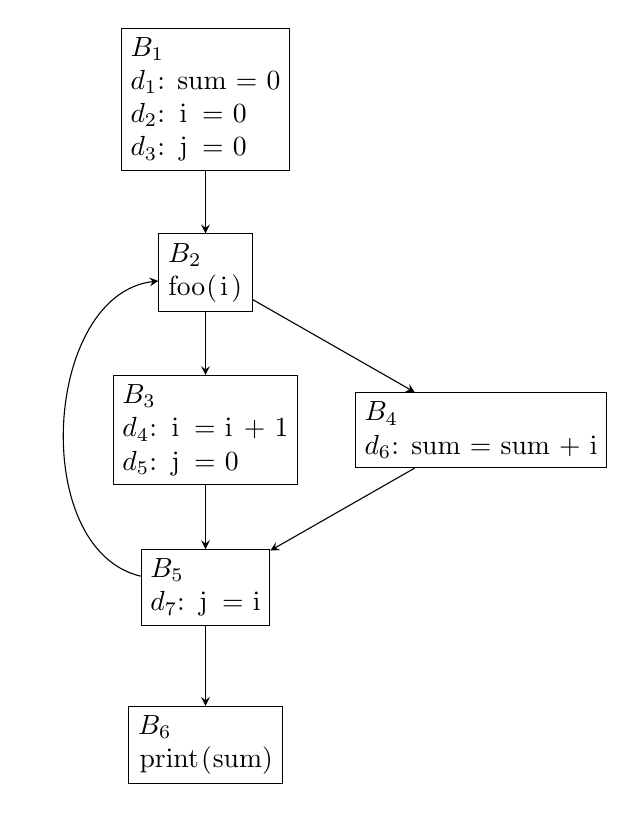
\begin{tikzpicture}[auto,
        ] 
        \tikzstyle{every node} = [ draw, align=left]
        \node (1) {$B_1$\\ $d_1$: \lstinline$sum = 0$\\ $d_2$: \lstinline$i = 0$\\ $d_3$: \lstinline$j = 0$ };
        \node [below of=1, node distance=2.2cm] (2) {$B_2$\\ \lstinline$foo(i)$ };
        \node [below  of=2, node distance=2cm] (3) {$B_3$\\ $d_4$: \lstinline$i = i + 1$\\ $d_5$: \lstinline$j = 0$};
        \node [right of=3, node distance=3.5cm] (4) {$B_4$\\ $d_6$: \lstinline$sum = sum + i$};
        \node [below of=3, node distance=2cm] (5) {$B_5$\\ $d_7$: \lstinline$j = i$};
        \node [below of=5, node distance=2cm] (6) {$B_6$\\ \lstinline$print(sum)$};
        
        \path (1) edge[cfgedge] (2); 
        \path (2) edge[cfgedge] (3);
        \path (2) edge[cfgedge] (4);
        \path (3) edge[cfgedge] (5);
        \path (4) edge[cfgedge] (5);
        \path (5) edge [cfgedge](6);
        \path (5) edge[cfgedge,bend left=80] (2);
        \end{tikzpicture}

        \lstinline$sum$ and \lstinline$i$ are \emph{Useful} at $OUT[B_1]$,
      while \lstinline$j$ is \emph{not Useful} at $OUT[B_1]$.


      Define the dataflow analysis that detects such \emph{Useful} variables.

      \begin{mdframed}
        Direction $D =$  % forward or backward

        Dataflow values $V = $  %TODO

        Meet operation $\wedge = $ %TODO

        Transfer functions $\mathcal{F}$ for each statement type including boundary conditions:  % TODO

      \end{mdframed}
      
      \clearpage
      \item (10 points)
      Let us define the \emph{Source-Flow problem} as follows:
      We say that the value of function \lstinline$source$ \emph{flows into} variable $x$ at program point $p$ if
      there exists a path from entry to $p$ on which $x$ was assigned the return value of a call to \lstinline$source$
      or $x$ was defined using a variable whose value flows from a call to \lstinline$source$,
      and then the variable $x$ was not modified along the path to point $p$.

      Consider the following control-flow graph:

      \begin{center}
      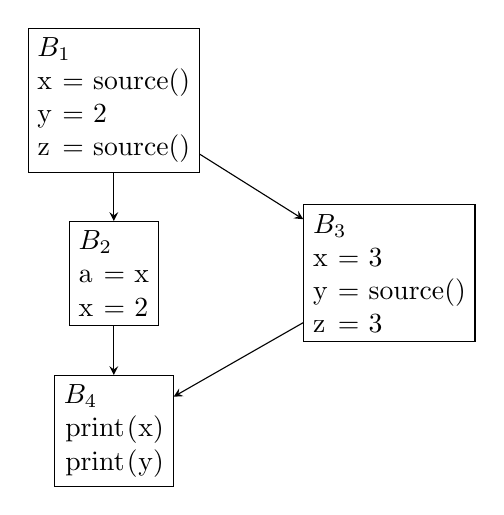
\begin{tikzpicture}[auto,
        ] 
        \tikzstyle{every node} = [ draw, align=left]
        \node (1) {$B_1$\\ \lstinline$x = source()$ \\ \lstinline$y = 2$\\ \lstinline$z = source()$};
        \node [below of=1, node distance=2.2cm] (2) {$B_2$\\ \lstinline $a = x$ \\ \lstinline$x = 2$ };
        \node [right of=2, node distance=3.5cm] (3) {$B_3$\\ \lstinline$x = 3$ \\ \lstinline$y = source()$ \\ \lstinline$z = 3$};
        \node [below of=2, node distance=2cm] (4) {$B_4$\\ \lstinline$print(x)$ \\ \lstinline$print(y)$};
        
        \path (1) edge[cfgedge] (2); 
        \path (1) edge[cfgedge] (3);
        \path (2) edge[cfgedge] (4);
        \path (3) edge[cfgedge] (4);
      \end{tikzpicture}
    \end{center}

      \lstinline$source()$ flows into variables $a$, $y$, and $z$, but does not
      flow into variable $x$ at $IN[B_4]$.

      Define the dataflow analysis for Source-Flow analysis.

      \begin{mdframed}
        Direction $D =$  % forward or backward %TODO

        Dataflow values $V = $  %TODO

        Meet operation $\wedge = $ %TODO

        Family of transfer functions $\mathcal{F}$ for each statement type
        including boundary conditions:  % TODO

      \end{mdframed}

      \item (5 points) Let the function $g: 2^{\{p,q,r, s\}} \rightarrow 2^{\{p,q,r,s\}}$ be defined 
      as $\lambda S. \{q, r\} \cup (S - \{p, q \})$. 
    
      Draw the \emph{representative relation} of $g$ as required by the IFDS framework:
    
      \begin{mdframed}
        \vspace{5em}
        %% TODO 
        
      \end{mdframed}

      \clearpage
      \item (10 points) This problem extends the notion of dominators in
      directed graphs to use the notion of CFL-reachability.

      Given an alphabet $\Sigma$, a \emph{labeled directed graph} $G(V, E, \phi)$ is a
      directed graph $G(V, E)$  along with a mapping $\phi \colon E \to \Sigma$,
      which maps each edge $e\in E$ to some label in the alphabet $\Sigma$. 

      Given a labeled directed graph $G(V, E, \phi)$ and a context-free language
      $L \subseteq \Sigma^*$, the sequence $v_1, v_2, \ldots, v_k$ is an
      \emph{$L$-path} from $v_1$ to $v_k$ iff $(v_i,v_{i+1}) \in E$, for every
      $1\leq i < k$ and the string $\phi((v_1, v_2)) \cdot \phi((v_2, v_3)) \cdot \ldots \cdot
      \phi((v_{k-1},v_k)) \in L$, where $\cdot$ is the concatenation operator. 

      Henceforth, assume that the graph $G$ has a unique start node that does
      not have any incoming edges. 

      A node $u$ \emph{$L$-dominates} a node $v$ iff all $L$-paths from start to 
      $v$ contain $u$. 

      A node $u$ \emph{strictly $L$-dominates} a node $v$ iff $u$ $L$-dominates $v$ 
      and $u \neq v$. 

      An \emph{immediate $L$-dominator} of a node $v$ is the last strict
      $L$-dominator of $v$ on some $L$-path from the entry to $v$. That is, $u$
      is an immediate $L$-dominator of a node $v$ if there exists an $L$-path
      $p$ from the entry to $v$ such that $u$ is the last strict dominator on
      $p$.

      State whether \textbf{True} or \textbf{False}: 
    
      \emph{Given a labeled directed graph $G(V,E, \phi)$ and a context-free
      language $L$, each node $n$ in $G$ has at most one immediate $L$-dominator.}

      In other words, the statement is saying that if $u$ is the last strict
      $L$-dominator on some path, then it implies that it is the last strict
      $L$-dominator on all paths. 
    
      If \textbf{True}, prove your answer. If \textbf{False}, provide an example
      of $G$ and $L$ and clearly state the node $n$ and its multiple immediate
      $L$-dominators.
      \begin{mdframed}
      \vspace{3em}
      %% TODO Comment out the correct answer.
      %\textbf{True} % Provide proof.
      %\textbf{False} % Provide counter example.
      \end{mdframed}
      
  \end{enumerate}
    
\end{document}
